\clearpage

\section{Data vs. MC Comparison in Preselection Region}
\label{sec:yields}

In this section we compare the data and MC samples passing the selection described in Sec.~\ref{sec:eventSelection}
In the following, the MC is reweighted to match the data distribution of number of reconstructed primary vertices.
%{\bf FIXME: UPDATE TO 5.1/fb VTX-REWEIGHTING, CURRENTLY USING OUTDATED FUNCTION}. 
The trigger efficiencies of Sec.~\ref{sec:datasets} are applied. In all plots, the last bin contains the overflow.

We begin by counting the inclusive Z yields. Here we require the presence of two selected leptons without
any additional requirements on jets or \MET. In Fig.~\ref{fig:dilmass} the distribution of dilepton invariant
mass in the ee and $\mu\mu$ channels is displayed. In Table~\ref{table:zyields} the yields for selected dilepton
events in the Z mass window are indicated. Good data vs. MC agreement is observed, within the systematic uncertainties
of integrated luminosity (4.5\%), trigger efficiency (3\%), \zjets\ and \ttbar\ cross sections.

\begin{figure}[hbt]
  \begin{center}
	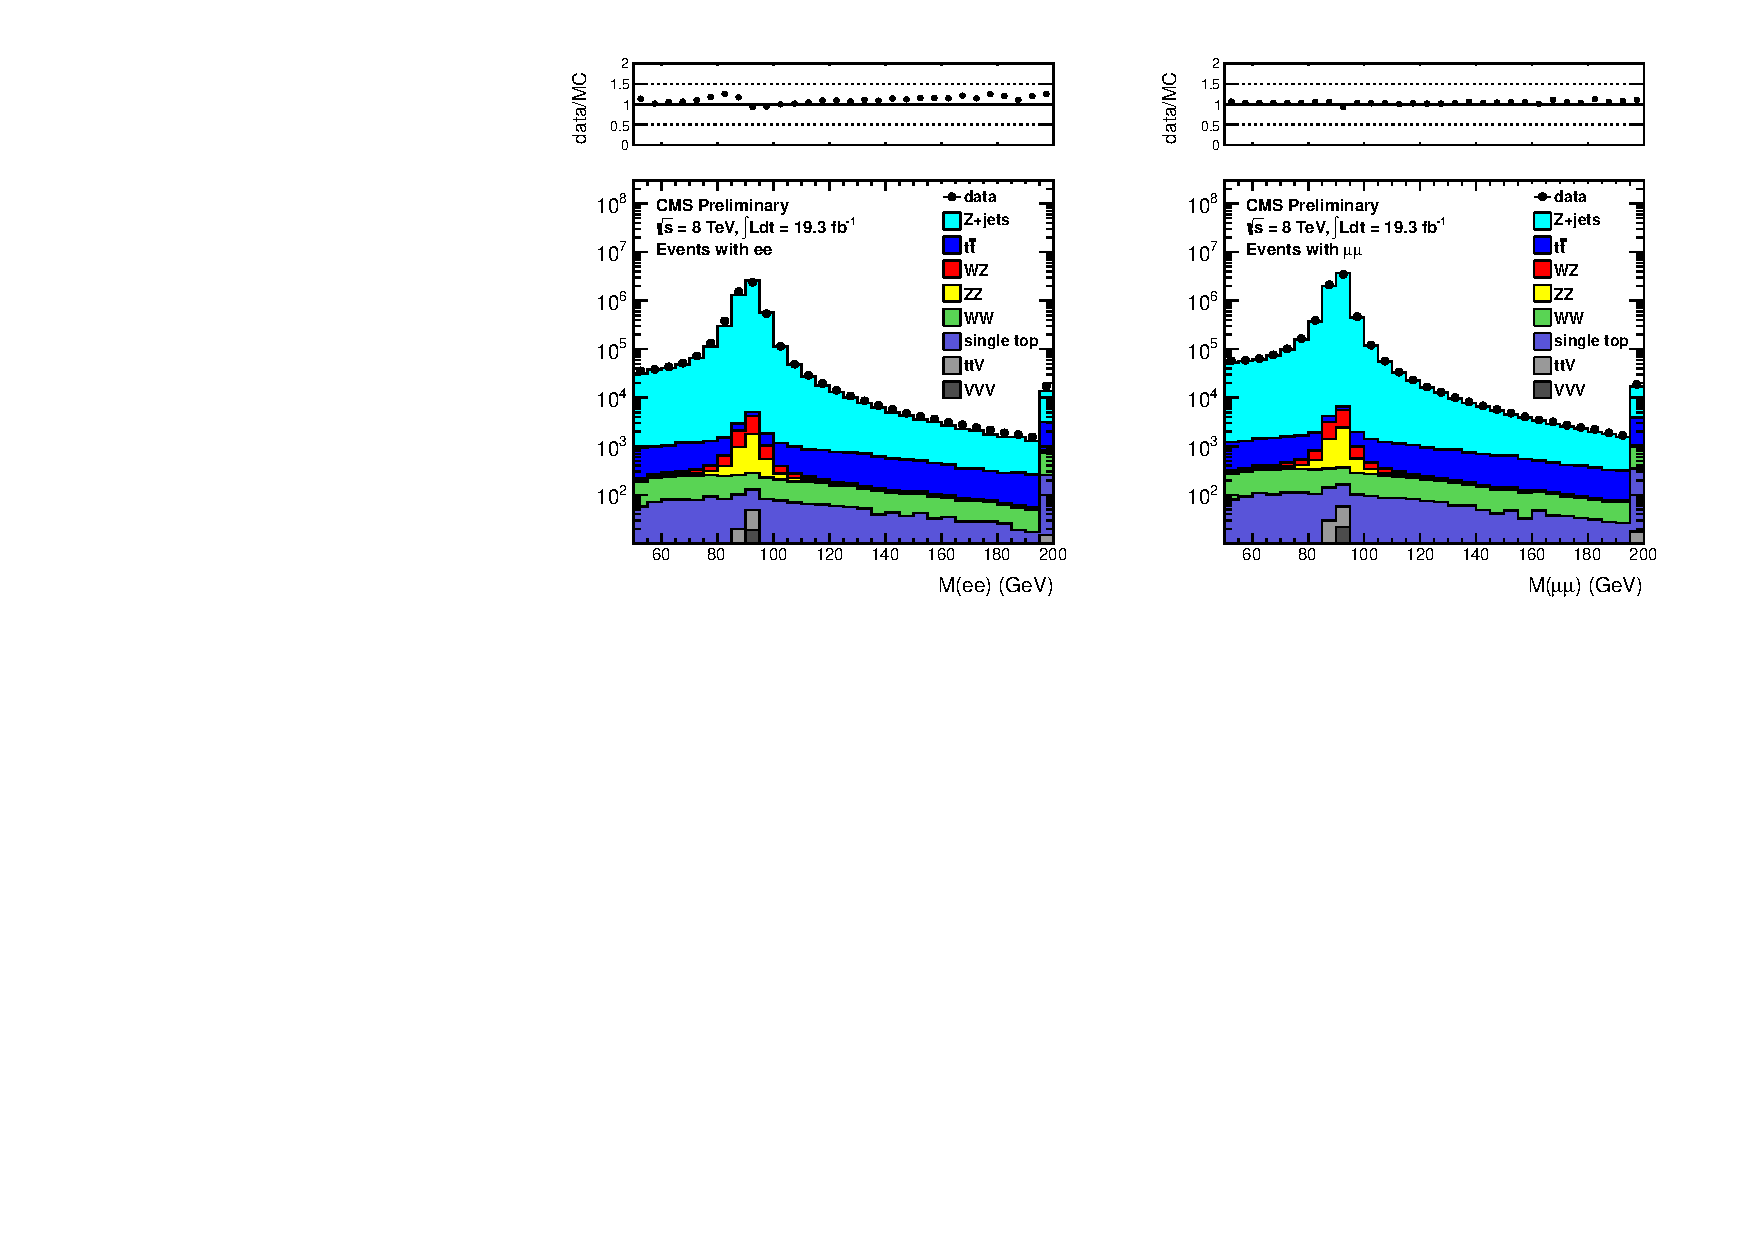
\includegraphics[width=1.0\linewidth]{plots/dilmass_19fb.pdf}
	\caption{
	  \label{fig:dilmass}\protect 
	  Dilepton mass distribution for events with two selected leptons
	  in the ee (left) and $\mu\mu$ (right) final states.}

%Loading babies at       : ../output/V00-02-00
%Using selection         : (((((leptype==0 && (ee==1 || isdata==0))||(leptype==1 && (mm==1 || isdata==0)))||(leptype==2 && (em==1||me==1||isdata==0)))&&(csc==0 && hbhe==1 && hcallaser==1 && ecaltp==1 && trkfail==1 && eebadsc==1 && hbhenew==1))&&(lep1.pt()>20.0 && lep2.pt()>20.0))&&(dilmass>15.0)
%Using weight            : weight * 19.3 * trgeff * vtxweight
%Plotting var dilmass flavor ee
%compareDataMC : apply trigeff 1
%MC yield VVV 42.68
%MC yield ttV 108.96
%MC yield single top 1779.47
%MC yield WW 3461.22
%MC yield ZZ 3069.20
%MC yield WZ 4971.64
%MC yield ttbar 18704.12
%SCALING ZJETS BY 111/946
%MC yield zjets 5335948.74
%MC total yield 5368086.00
%data yield 5.51894e+06
%Plotting var dilmass flavor mm
%compareDataMC : apply trigeff 1
%Warning in <TROOT::Append>: Replacing existing TH1: htemp (Potential memory leak).
%MC yield VVV 53.17
%MC yield ttV 134.87
%MC yield single top 2306.47
%MC yield WW 4582.01
%MC yield ZZ 4032.27
%MC yield WZ 6456.02
%MC yield ttbar 23381.81
%SCALING ZJETS BY 111/946
%MC yield zjets 7324507.81
%MC total yield 7365454.50
%data yield 7.31115e+06

  \end{center}
\end{figure}


\begin{table}[htb]
\begin{center}
\caption{\label{table:zyields} Data and Monte Carlo yields for events with two selected leptons in the Z mass window. }
\begin{tabular}{lccccc}

%Loading babies at       : ../output/V00-02-00
%Using selection         : ((((((leptype==0 && (ee==1 || isdata==0))||(leptype==1 && (mm==1 || isdata==0)))||(leptype==2 && (em==1||me==1||isdata==0)))&&(csc==0 && hbhe==1 && hcallaser==1 && ecaltp==1 && trkfail==1 && eebadsc==1 && hbhenew==1))&&(lep1.pt()>20.0 && lep2.pt()>20.0))&&(dilmass>15.0))&&(dilmass>81 && dilmass<101)
%Using weight            : weight * 19.3 * trgeff * vtxweight


\hline
\hline
         Sample   &             ee   &       $\mu\mu$   &         e$\mu$   &          total  \\
\hline
%SCALING ZJETS BY 111/946
         \zjets   &4735966.0 $\pm$ 3483.0   &6507980.5 $\pm$ 3928.4   &2270.5 $\pm$ 75.1   &11246217.0 $\pm$ 5250.7  \\
         \ttbar   &3312.7 $\pm$ 47.4   &4192.1 $\pm$ 51.2   &7535.8 $\pm$ 70.3   &15040.6 $\pm$ 99.0  \\
             WZ   &4306.1 $\pm$ 7.5   &5647.2 $\pm$ 8.3   &113.5 $\pm$ 1.1   &10066.8 $\pm$ 11.2  \\
             ZZ   &2713.5 $\pm$ 5.7   &3582.7 $\pm$ 6.2   & 10.8 $\pm$ 0.1   &6307.0 $\pm$ 8.4  \\
             WW   &609.5 $\pm$ 6.2   &812.3 $\pm$ 6.8   &1408.2 $\pm$ 9.2   &2830.0 $\pm$ 13.0  \\
     single top   &314.6 $\pm$ 12.3   &404.1 $\pm$ 13.3   &698.4 $\pm$ 18.0   &1417.0 $\pm$ 25.5  \\
            ttV   & 56.6 $\pm$ 1.1   & 69.9 $\pm$ 1.2   & 21.3 $\pm$ 0.7   &147.8 $\pm$ 1.7  \\
            VVV   & 26.3 $\pm$ 0.3   & 33.3 $\pm$ 0.4   &  6.8 $\pm$ 0.2   & 66.3 $\pm$ 0.6  \\
\hline
    total SM MC   &4747305.0 $\pm$ 3483.4   &6522722.0 $\pm$ 3928.8   &12065.3 $\pm$ 104.8   &11282092.3 $\pm$ 5251.7  \\
\hline
           data   &        4828868   &        6434546   &          12872   &       11276286  \\
\hline
\hline

\end{tabular}
\end{center}
\end{table}

\clearpage

We next define the preselection region for the inclusive search using the following requirements:
\begin{itemize}
\item Number of jets $\geq$ 2;
\item Same flavor dileptons (opposite flavor yields will be shown since they are used in data for the FS background estimation);
\item Dilepton invariant mass $81<m_{\ell\ell}<101$ GeV.
\end{itemize}

The dilepton mass distributions in the preselection region of the inclusive search (without the dilepton mass requirement applied) 
for the ee and $\mu\mu$ final states are shown in Figure~\ref{fig:dilmass_2j}. In Table~\ref{table:zyields_2j} the data and MC yields 
in the inclusive preselection region are indicated. Good data vs. MC agreement is observed.


\begin{figure}[hbt]
  \begin{center}
	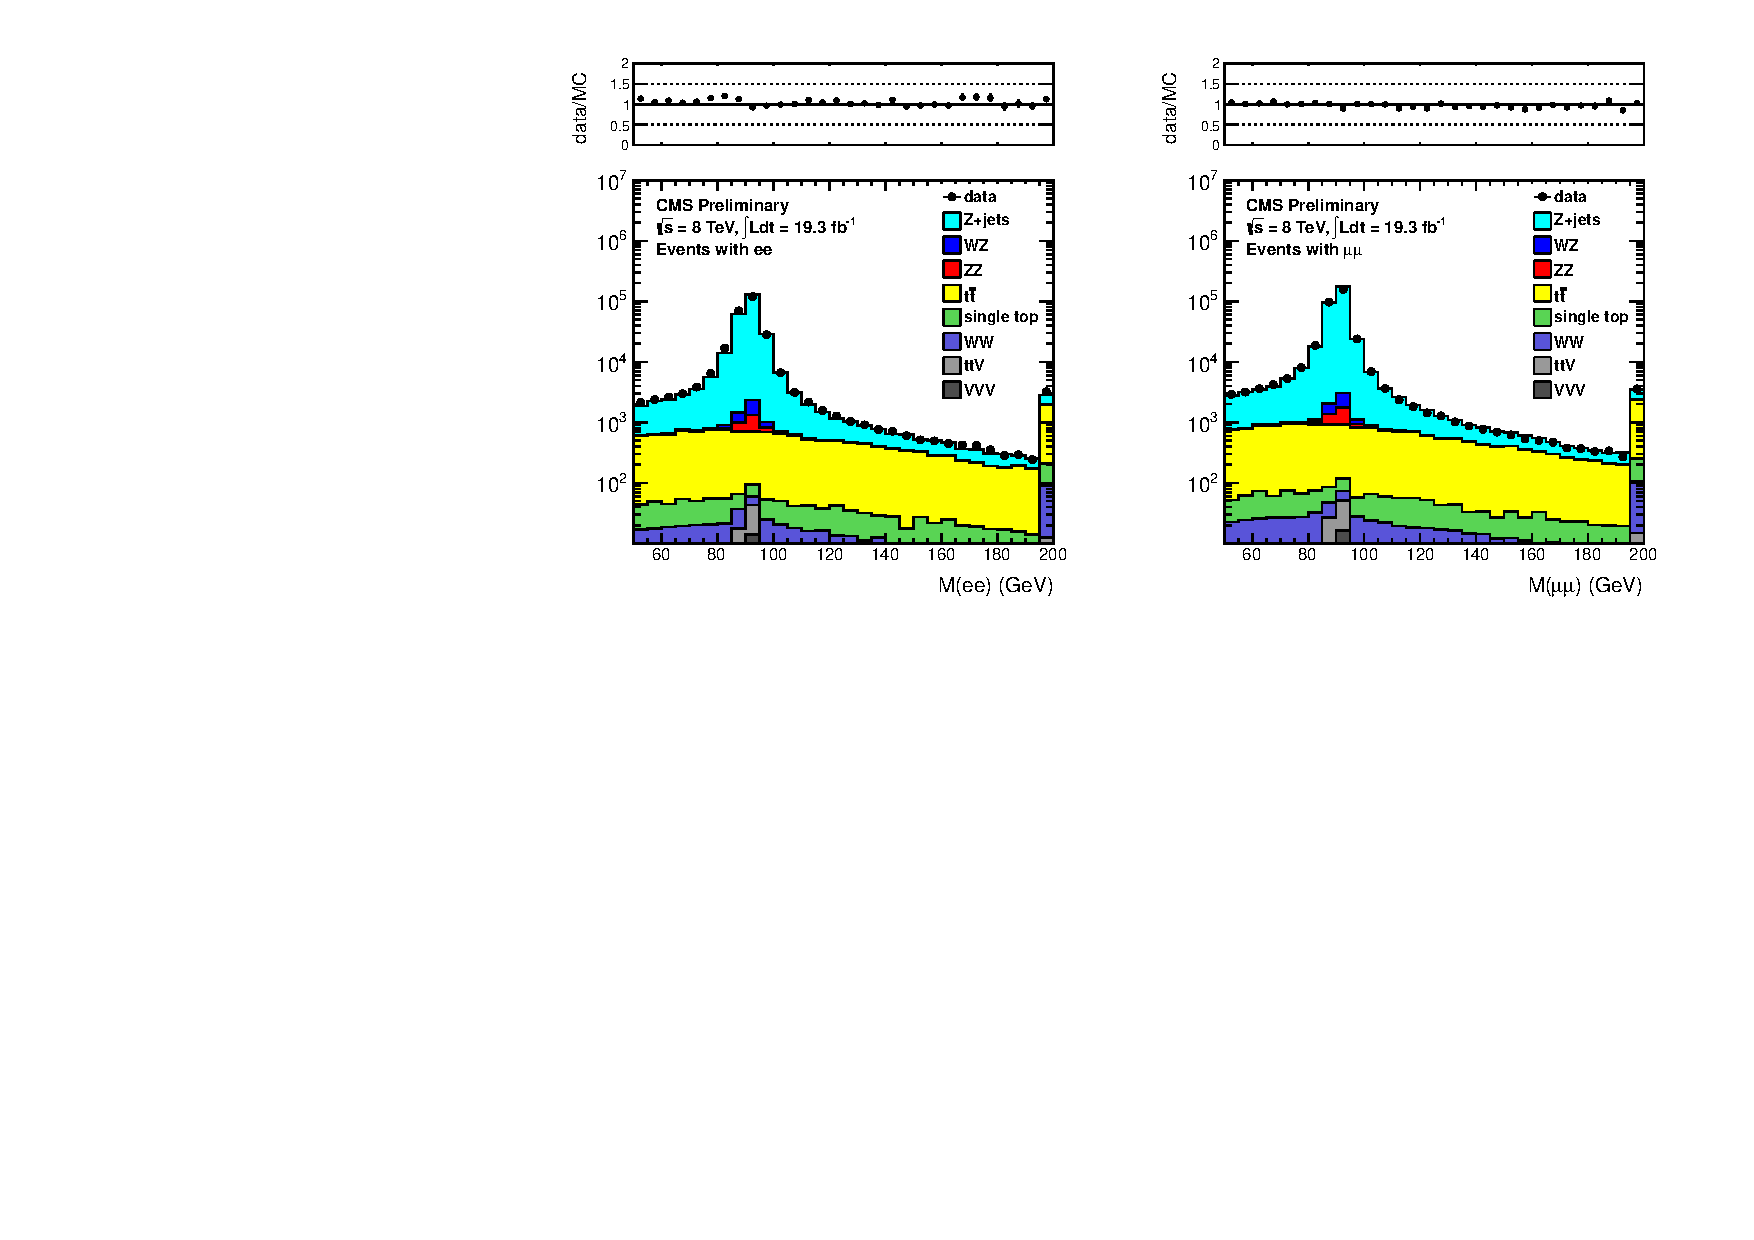
\includegraphics[width=1.0\linewidth]{plots/dilmass_2jets_19fb.pdf}
	\caption{
	  \label{fig:dilmass_2j}\protect 
	  Dilepton mass distribution for events in the preselection region of the inclusive search
	  in the ee (left) and $\mu\mu$ (right) final states.}


%Loading babies at       : ../output/V00-02-00
%-------------------------------------
%USING SKIMMED SAMPLES WITH NJETS >= 2
%-------------------------------------

%Using selection         : ((((((leptype==0 && (ee==1 || isdata==0))||(leptype==1 && (mm==1 || isdata==0)))||(leptype==2 && (em==1||me==1||isdata==0)))&&(csc==0 && hbhe==1 && hcallaser==1 && ecaltp==1 && trkfail==1 && eebadsc==1 && hbhenew==1))&&(lep1.pt()>20.0 && lep2.pt()>20.0))&&(dilmass>15.0))&&(njets>=2)
%Using weight            : weight * 19.3 * trgeff * vtxweight
%Plotting var dilmass flavor ee
%compareDataMC : apply trigeff 1
%MC yield VVV 28.97
%MC yield ttV 102.80
%MC yield single top 758.68
%MC yield WW 418.46
%MC yield ZZ 1260.58
%MC yield WZ 2051.00
%MC yield ttbar 14406.73
%SCALING ZJETS BY 111/946
%MC yield zjets 257952.20
%MC total yield 276979.41
%data yield 286743
%Plotting var dilmass flavor mm
%compareDataMC : apply trigeff 1
%Warning in <TROOT::Append>: Replacing existing TH1: htemp (Potential memory leak).
%MC yield VVV 35.94
%MC yield ttV 128.07
%MC yield single top 970.44
%MC yield WW 538.01
%MC yield ZZ 1633.77
%MC yield WZ 2626.89
%MC yield ttbar 18006.61
%SCALING ZJETS BY 111/946
%MC yield zjets 345766.46
%MC total yield 369706.19
%data yield 362279


  \end{center}
\end{figure}

\begin{table}[htb]
\begin{center}
\caption{\label{table:zyields_2j} Data and MC yields in the preselection region of the inclusive search.
}
\begin{tabular}{lccccc}

%Loading babies at       : ../output/V00-02-00
%-------------------------------------
%USING SKIMMED SAMPLES WITH NJETS >= 2
%-------------------------------------

%Using selection         : (((((((leptype==0 && (ee==1 || isdata==0))||(leptype==1 && (mm==1 || isdata==0)))||(leptype==2 && (em==1||me==1||isdata==0)))&&(csc==0 && hbhe==1 && hcallaser==1 && ecaltp==1 && trkfail==1 && eebadsc==1 && hbhenew==1))&&(lep1.pt()>20.0 && lep2.pt()>20.0))&&(dilmass>15.0))&&(njets>=2))&&(dilmass>81 && dilmass<101)
%Using weight            : weight * 19.3 * trgeff * vtxweight


\hline
\hline
         Sample   &             ee   &       $\mu\mu$   &         e$\mu$   &          total  \\
\hline
%SCALING ZJETS BY 111/946
         \zjets   &228270.2 $\pm$ 751.0   &306348.9 $\pm$ 836.3   &125.3 $\pm$ 17.5   &534744.4 $\pm$ 1124.2  \\
         \ttbar   &2561.2 $\pm$ 41.6   &3240.6 $\pm$ 45.0   &5849.1 $\pm$ 61.8   &11650.9 $\pm$ 87.1  \\
             WZ   &1790.4 $\pm$ 4.9   &2308.4 $\pm$ 5.4   & 22.4 $\pm$ 0.5   &4121.2 $\pm$ 7.3  \\
             ZZ   &1116.9 $\pm$ 3.8   &1453.3 $\pm$ 4.2   &  2.5 $\pm$ 0.1   &2572.7 $\pm$ 5.6  \\
             WW   & 68.6 $\pm$ 2.1   & 89.1 $\pm$ 2.3   &156.7 $\pm$ 3.0   &314.4 $\pm$ 4.3  \\
     single top   &126.7 $\pm$ 7.7   &153.4 $\pm$ 8.2   &276.4 $\pm$ 11.2   &556.6 $\pm$ 15.9  \\
            ttV   & 54.4 $\pm$ 1.1   & 67.5 $\pm$ 1.1   & 19.7 $\pm$ 0.7   &141.6 $\pm$ 1.7  \\
            VVV   & 19.3 $\pm$ 0.3   & 24.4 $\pm$ 0.3   &  3.4 $\pm$ 0.1   & 47.1 $\pm$ 0.5  \\
\hline
    total SM MC   &234007.8 $\pm$ 752.3   &313685.7 $\pm$ 837.6   &6455.5 $\pm$ 65.3   &554149.1 $\pm$ 1127.7  \\
\hline
           data   &         239661   &         304953   &           6279   &         550893  \\
\hline
\hline


\end{tabular}
\end{center}
\end{table}


\clearpage

We next define the preselection region for the targeted search by adding the following requirements:
\begin{itemize}
\item Veto events containing a b-tagged jet;
\item Dijet invariant mass $70<m_{jj}<110$ GeV;
\item Veto events containing a third selected lepton (electron or muon) with \pt $>$ 10 GeV; 
\end{itemize}

The rejection of events with a b-tagged jet strongly suppresses the \ttbar\ background, which is the dominant background in the inclusive search
after requiring large \MET. The requirement that the jet pair is consistent with originating from W/Z decay is motivated by the fact that we are 
searching for signatures producing V(jj)Z($\ell\ell$)+\MET; this requirement suppresses the \zjets\ and \ttbar\ backgrounds. The veto of events
containting a third electron or muon suppresses the WZ background, and also serves to make this analyis exclusive with respect to searches in
the trilepton final state.

The dilepton mass distributions in the preselection region of the targeted search (without the dilepton mass requirement applied) 
for the ee and $\mu\mu$ final states are shown in Figure~\ref{fig:dilmass_2j_targeted}. In Table~\ref{table:zyields_2j_targeted} 
the data and MC yields in the preselection region are indicated. Good data vs. MC agreement is observed.
We also show the distribution of dijet mass in the targeted preselection (with the requirement on this quantity removed) in Fig.~\ref{fig:mjj},
which demonstrates that the MC does a reasonable job of modeling this quantity.

%-------------------------------------
% veto b-jets with CSV MEDIUM 
%-------------------------------------

\begin{figure}[hbt]
  \begin{center}
	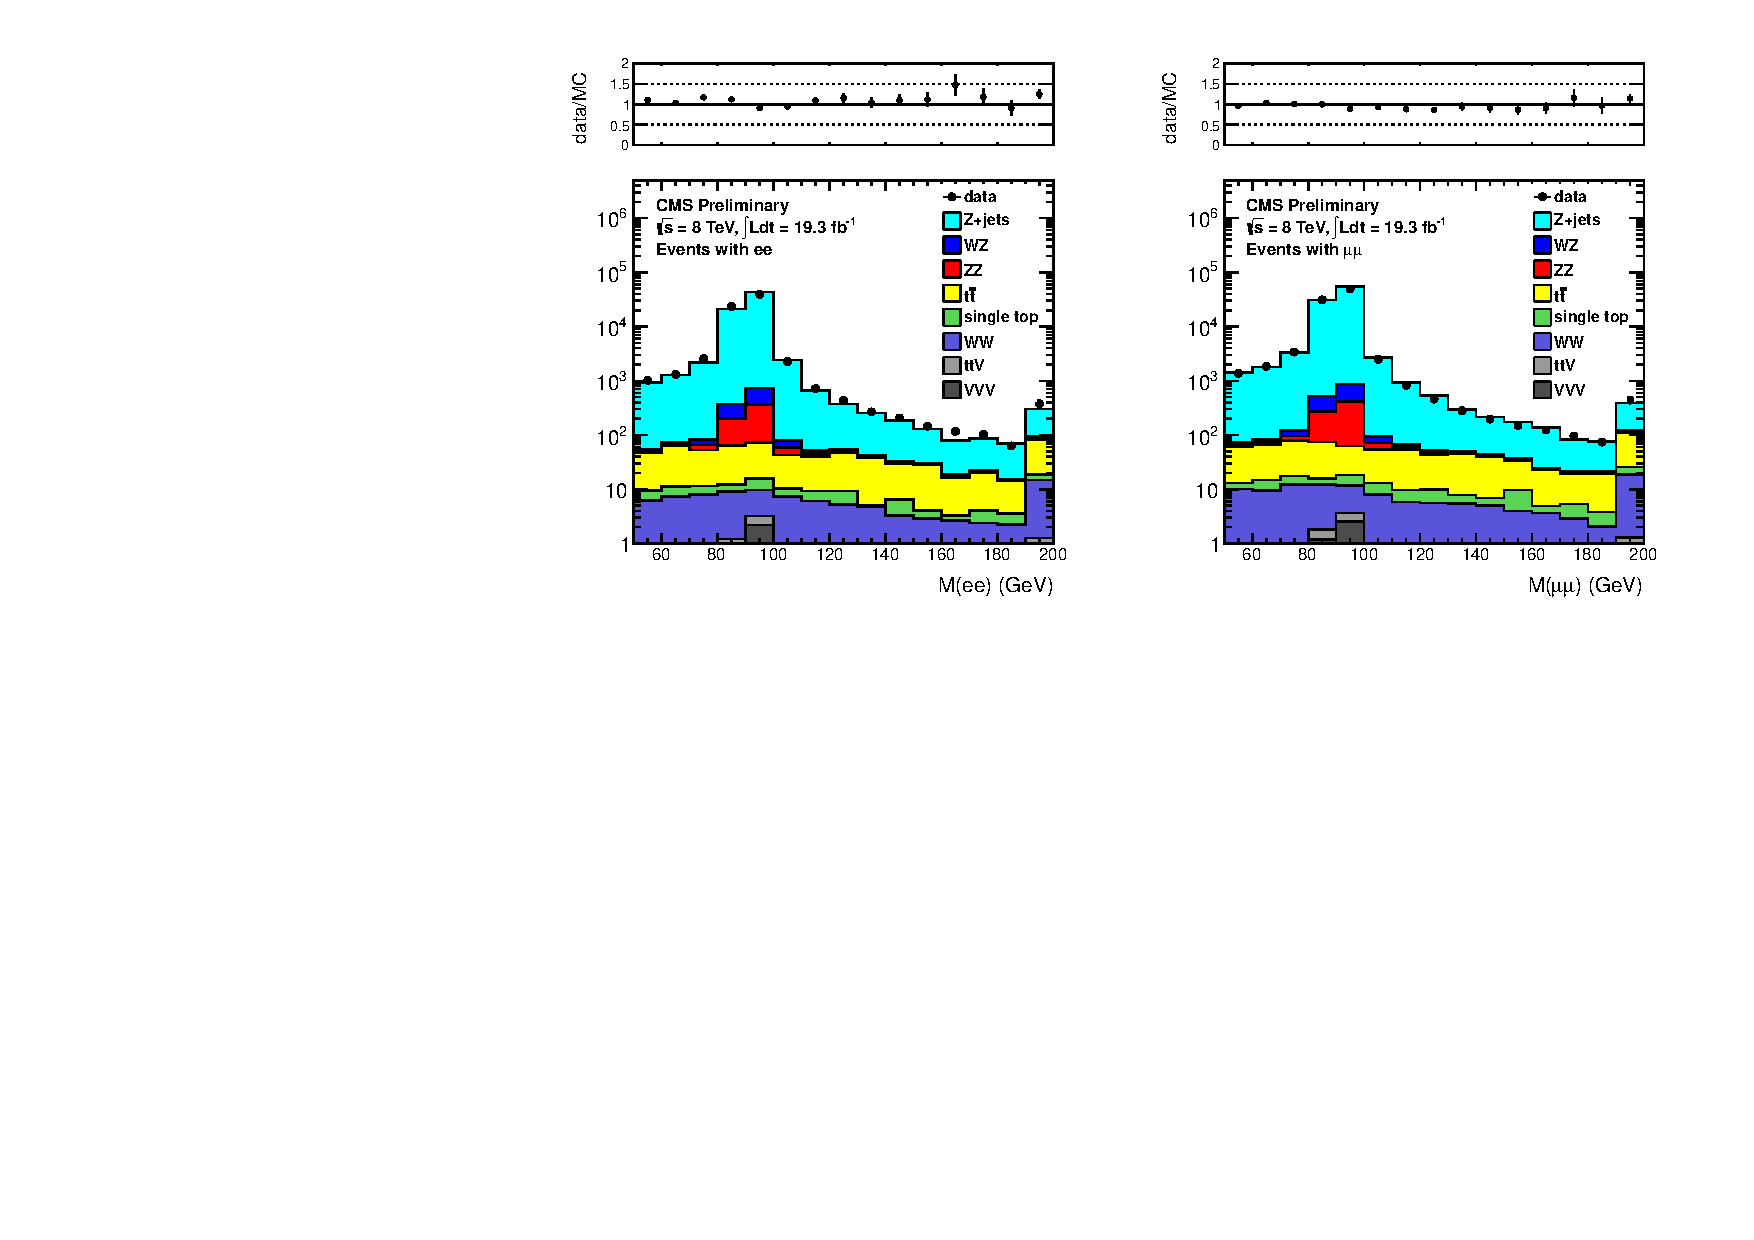
\includegraphics[width=1.0\linewidth]{plots/dilmass_targeted_19fb.pdf}
	\caption{
	  \label{fig:dilmass_2j_targeted}\protect 
	  Dilepton mass distribution for events in the preselection region of the targeted search
	  in the ee (left) and $\mu\mu$ (right) final states.}


%Loading babies at       : ../output/V00-02-00
%-------------------------------------
%USING SKIMMED SAMPLES WITH NJETS >= 2
%-------------------------------------

%Using selection         : (((((((((leptype==0 && (ee==1 || isdata==0))||(leptype==1 && (mm==1 || isdata==0)))||(leptype==2 && (em==1||me==1||isdata==0)))&&(csc==0 && hbhe==1 && hcallaser==1 && ecaltp==1 && trkfail==1 && eebadsc==1 && hbhenew==1))&&(lep1.pt()>20.0 && lep2.pt()>20.0))&&(dilmass>15.0))&&(njets>=2))&&(nbcsvm==0))&&(mjj>70.0 && mjj<110.0))&&(nlep==2)
%Using weight            : weight * 19.3 * trgeff * vtxweight
%Plotting var dilmass flavor ee
%compareDataMC : apply trigeff 1
%MC yield VVV 5.25
%MC yield ttV 3.50
%MC yield single top 43.11
%MC yield WW 83.00
%MC yield ZZ 482.09
%MC yield WZ 623.38
%MC yield ttbar 527.48
%SCALING ZJETS BY 111/946
%MC yield zjets 71286.31
%MC total yield 73054.11
%data yield 74303
%Plotting var dilmass flavor mm
%compareDataMC : apply trigeff 1
%Warning in <TROOT::Append>: Replacing existing TH1: htemp (Potential memory leak).
%MC yield VVV 6.58
%MC yield ttV 3.59
%MC yield single top 58.93
%MC yield WW 107.13
%MC yield ZZ 622.74
%MC yield WZ 808.68
%MC yield ttbar 607.63
%SCALING ZJETS BY 111/946
%MC yield zjets 96483.36
%MC total yield 98698.63
%data yield 94596

  \end{center}
\end{figure}

\begin{table}[htb]
\begin{center}
\caption{\label{table:zyields_2j_targeted} Data and MC yields in the preselection region of the targeted search.
}
\begin{tabular}{lccccc}

%Loading babies at       : ../output/V00-02-00
%-------------------------------------
%USING SKIMMED SAMPLES WITH NJETS >= 2
%-------------------------------------

%Using selection         : ((((((((((leptype==0 && (ee==1 || isdata==0))||(leptype==1 && (mm==1 || isdata==0)))||(leptype==2 && (em==1||me==1||isdata==0)))&&(csc==0 && hbhe==1 && hcallaser==1 && ecaltp==1 && trkfail==1 && eebadsc==1 && hbhenew==1))&&(lep1.pt()>20.0 && lep2.pt()>20.0))&&(dilmass>15.0))&&(njets>=2))&&(nbcsvm==0))&&(mjj>70.0 && mjj<110.0))&&(nlep==2))&&(dilmass>81 && dilmass<101)
%Using weight            : weight * 19.3 * trgeff * vtxweight


\hline
\hline
         Sample   &             ee   &       $\mu\mu$   &         e$\mu$   &          total  \\
\hline
%SCALING ZJETS BY 111/946
         \zjets   &63014.6 $\pm$ 392.2   &85083.6 $\pm$ 438.2   & 27.1 $\pm$ 7.8   &148125.3 $\pm$ 588.1  \\
         \ttbar   &106.0 $\pm$ 8.5   &102.9 $\pm$ 7.9   &220.5 $\pm$ 12.0   &429.4 $\pm$ 16.7  \\
             WZ   &546.8 $\pm$ 2.8   &712.9 $\pm$ 3.0   &  3.5 $\pm$ 0.2   &1263.2 $\pm$ 4.1  \\
             ZZ   &428.3 $\pm$ 2.4   &554.0 $\pm$ 2.6   &  0.4 $\pm$ 0.1   &982.7 $\pm$ 3.5  \\
             WW   & 14.2 $\pm$ 0.9   & 18.0 $\pm$ 1.0   & 33.4 $\pm$ 1.4   & 65.6 $\pm$ 2.0  \\
     single top   &  9.8 $\pm$ 2.2   & 10.5 $\pm$ 2.1   & 17.8 $\pm$ 2.8   & 38.1 $\pm$ 4.2  \\
            ttV   &  1.6 $\pm$ 0.2   &  1.7 $\pm$ 0.2   &  0.9 $\pm$ 0.1   &  4.2 $\pm$ 0.3  \\
            VVV   &  2.9 $\pm$ 0.1   &  3.7 $\pm$ 0.1   &  0.9 $\pm$ 0.1   &  7.5 $\pm$ 0.2  \\
\hline
    total SM MC   &64124.2 $\pm$ 392.3   &86487.3 $\pm$ 438.3   &304.5 $\pm$ 14.7   &150916.0 $\pm$ 588.4  \\
\hline
           data   &          64385   &          82426   &            306   &         147117  \\
\hline
\hline

\end{tabular}
\end{center}
\end{table}



\begin{comment}

%-------------------------------------
% veto b-jets with CSV LOOSE 
%-------------------------------------

\begin{figure}[hbt]
  \begin{center}
	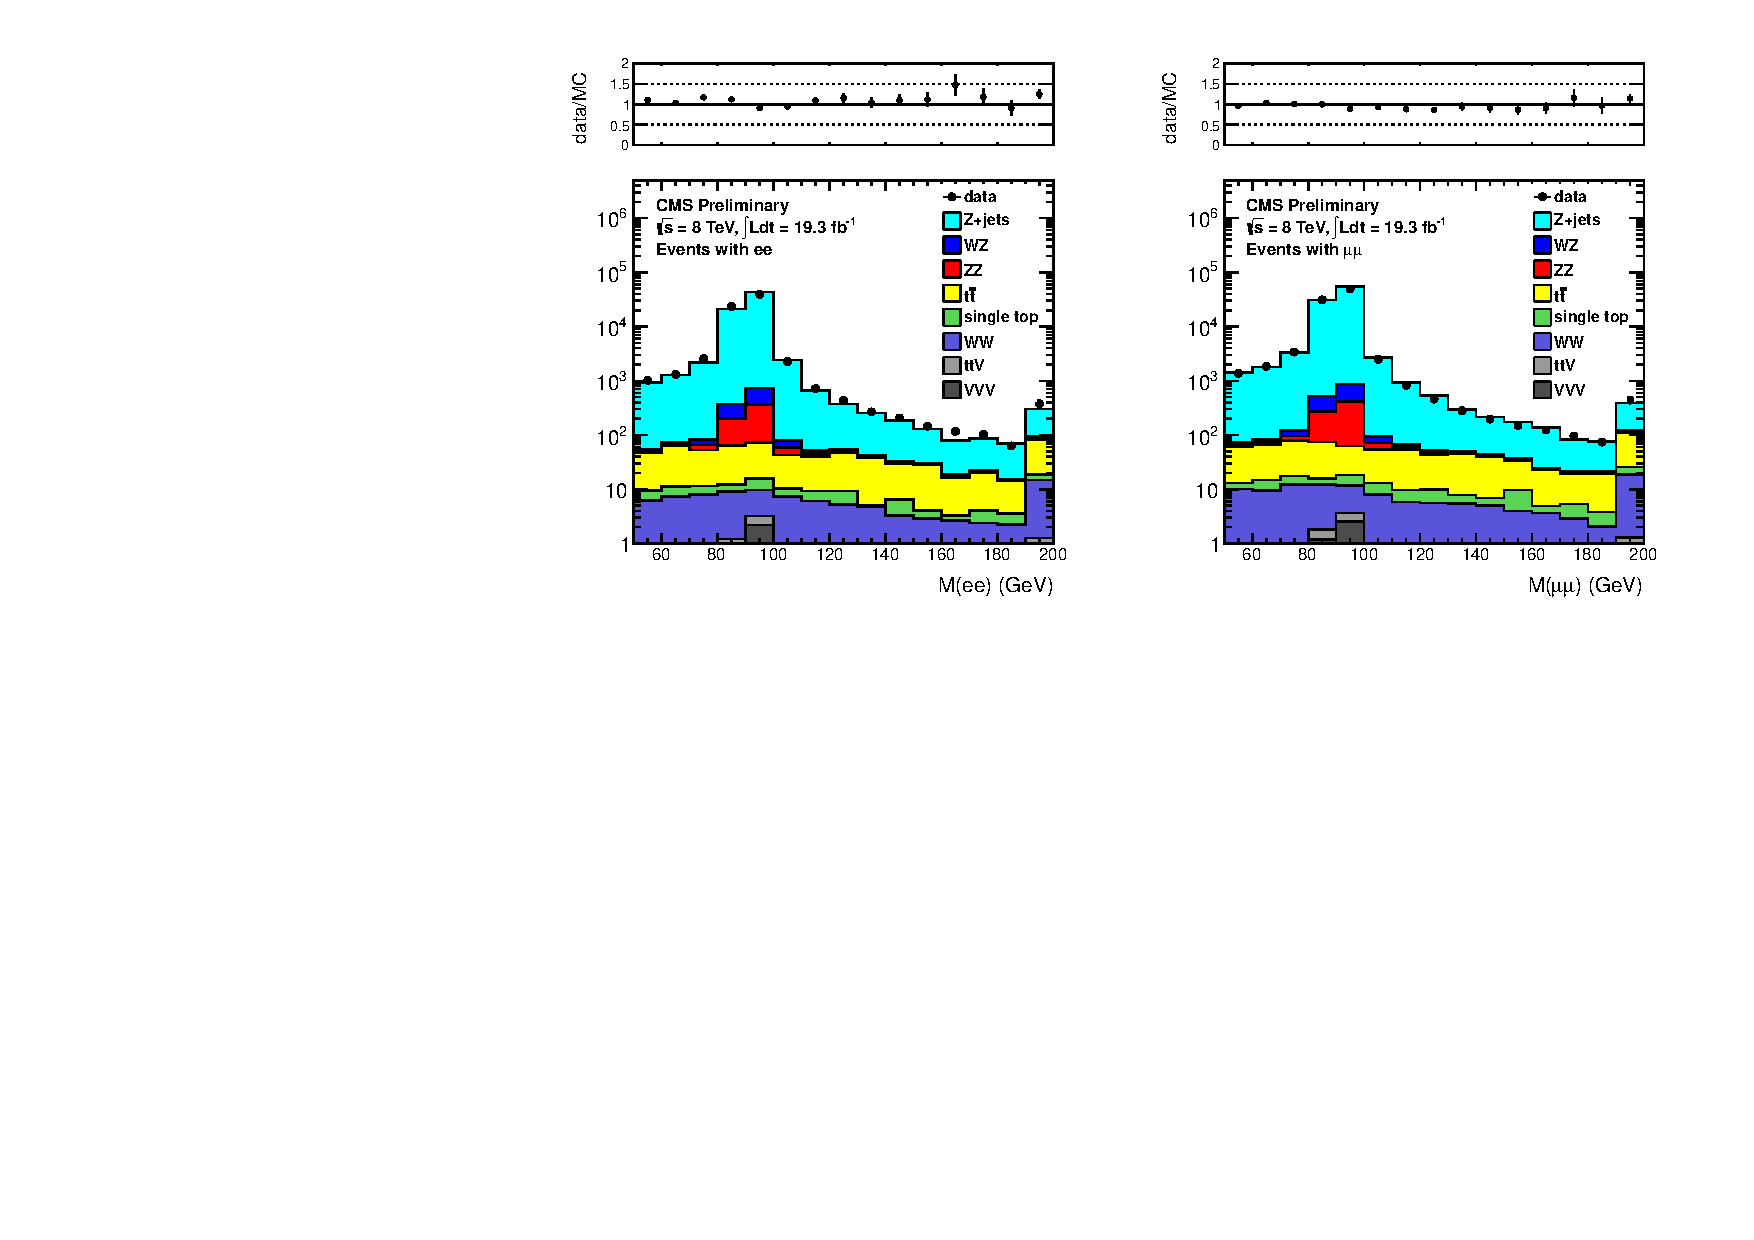
\includegraphics[width=1.0\linewidth]{plots/dilmass_targeted_19fb.pdf}
	\caption{
	  \label{fig:dilmass_2j_targeted}\protect 
	  Dilepton mass distribution for events in the preselection region of the targeted search
	  in the ee (left) and $\mu\mu$ (right) final states.}

%Loading babies at       : ../output/V00-01-04
%-------------------------------------
%USING SKIMMED SAMPLES WITH NJETS >= 2
%-------------------------------------

%Using selection         : ((((((((isdata==0 || (run<197556 || run>198913))&&(((leptype==0 && (ee==1 || isdata==0))||(leptype==1 && (mm==1 || isdata==0)))||(leptype==2 && (em==1||me==1||isdata==0))))&&(csc==0 && hbhe==1 && hcallaser==1 && ecaltp==1 && trkfail==1 && eebadsc==1 && hbhenew==1))&&(lep1.pt()>20.0 && lep2.pt()>20.0))&&(dilmass>15.0))&&(njets>=2))&&(nbcsvl==0))&&(mjj>70.0 && mjj<110.0))&&(nlep==2)
%Using weight            : weight * 9.2 * trgeff * vtxweight
%Plotting var dilmass flavor ee
%compareDataMC : apply trigeff 1
%MC yield VVV 1.69
%MC yield ttV 0.71
%MC yield WW 29.99
%MC yield single top 10.71
%MC yield ttbar 98.96
%MC yield ZZ 160.28
%MC yield WZ 201.63
%SCALING ZJETS BY 111/946
%MC yield zjets 26365.25
%MC total yield 26869.22
%data yield 24722
%Plotting var dilmass flavor mm
%compareDataMC : apply trigeff 1
%Warning in <TROOT::Append>: Replacing existing TH1: htemp (Potential memory leak).
%MC yield VVV 2.05
%MC yield ttV 0.70
%MC yield WW 38.74
%MC yield single top 13.48
%MC yield ttbar 104.95
%MC yield ZZ 206.22
%MC yield WZ 262.27
%SCALING ZJETS BY 111/946
%MC yield zjets 35489.85
%MC total yield 36118.25
%data yield 32393

  \end{center}
\end{figure}

\begin{table}[htb]
\begin{center}
\caption{\label{table:zyields_2j_targeted} Data and MC yields in the preselection region of the inclusive search.
}
\begin{tabular}{lccccc}
\hline
\hline
         Sample   &           ee   &       $\mu\mu$   &         e$\mu$   &            total  \\
\hline

%Loading babies at       : ../output/V00-01-04
%-------------------------------------
%USING SKIMMED SAMPLES WITH NJETS >= 2
%-------------------------------------

%Using selection         : (((((((((isdata==0 || (run<197556 || run>198913))&&(((leptype==0 && (ee==1 || isdata==0))||(leptype==1 && (mm==1 || isdata==0)))||(leptype==2 && (em==1||me==1||isdata==0))))&&(csc==0 && hbhe==1 && hcallaser==1 && ecaltp==1 && trkfail==1 && eebadsc==1 && hbhenew==1))&&(lep1.pt()>20.0 && lep2.pt()>20.0))&&(dilmass>15.0))&&(njets>=2))&&(nbcsvl==0))&&(mjj>70.0 && mjj<110.0))&&(nlep==2))&&(dilmass>81 && dilmass<101)
%Using weight            : weight * 9.2 * trgeff * vtxweight

\hline
         Sample   &           $ee$   &       $\mu\mu$   &         $e\mu$   &            tot  \\
\hline
SCALING ZJETS BY 111/946
          zjets   &23338.4 $\pm$ 164.1   &31251.5 $\pm$ 182.6   &  8.9 $\pm$ 3.1   &54598.8 $\pm$ 245.5  \\
             WZ   &176.4 $\pm$ 1.1   &231.1 $\pm$ 1.2   &  1.1 $\pm$ 0.1   &408.7 $\pm$ 1.6  \\
             ZZ   &142.3 $\pm$ 0.9   &183.2 $\pm$ 1.0   &  0.1 $\pm$ 0.0   &325.6 $\pm$ 1.4  \\
          ttbar   & 20.6 $\pm$ 2.5   & 15.5 $\pm$ 2.1   & 38.1 $\pm$ 3.4   & 74.2 $\pm$ 4.7  \\
     single top   &  2.3 $\pm$ 0.7   &  2.9 $\pm$ 0.7   &  4.5 $\pm$ 1.0   &  9.6 $\pm$ 1.4  \\
             WW   &  5.0 $\pm$ 0.4   &  6.8 $\pm$ 0.4   & 12.3 $\pm$ 0.6   & 24.2 $\pm$ 0.8  \\
            ttV   &  0.3 $\pm$ 0.1   &  0.3 $\pm$ 0.1   &  0.2 $\pm$ 0.0   &  0.8 $\pm$ 0.1  \\
            VVV   &  0.9 $\pm$ 0.0   &  1.1 $\pm$ 0.0   &  0.3 $\pm$ 0.0   &  2.3 $\pm$ 0.1  \\
\hline
      tot SM MC   &23686.1 $\pm$ 164.1   &31692.4 $\pm$ 182.6   & 65.7 $\pm$ 4.7   &55444.2 $\pm$ 245.5  \\
\hline
           data   &          21529   &          28265   &             53   &          49847  \\
\hline
\hline

\end{tabular}
\end{center}
\end{table}

\end{comment}


\clearpage

\begin{figure}[hbt]
  \begin{center}
	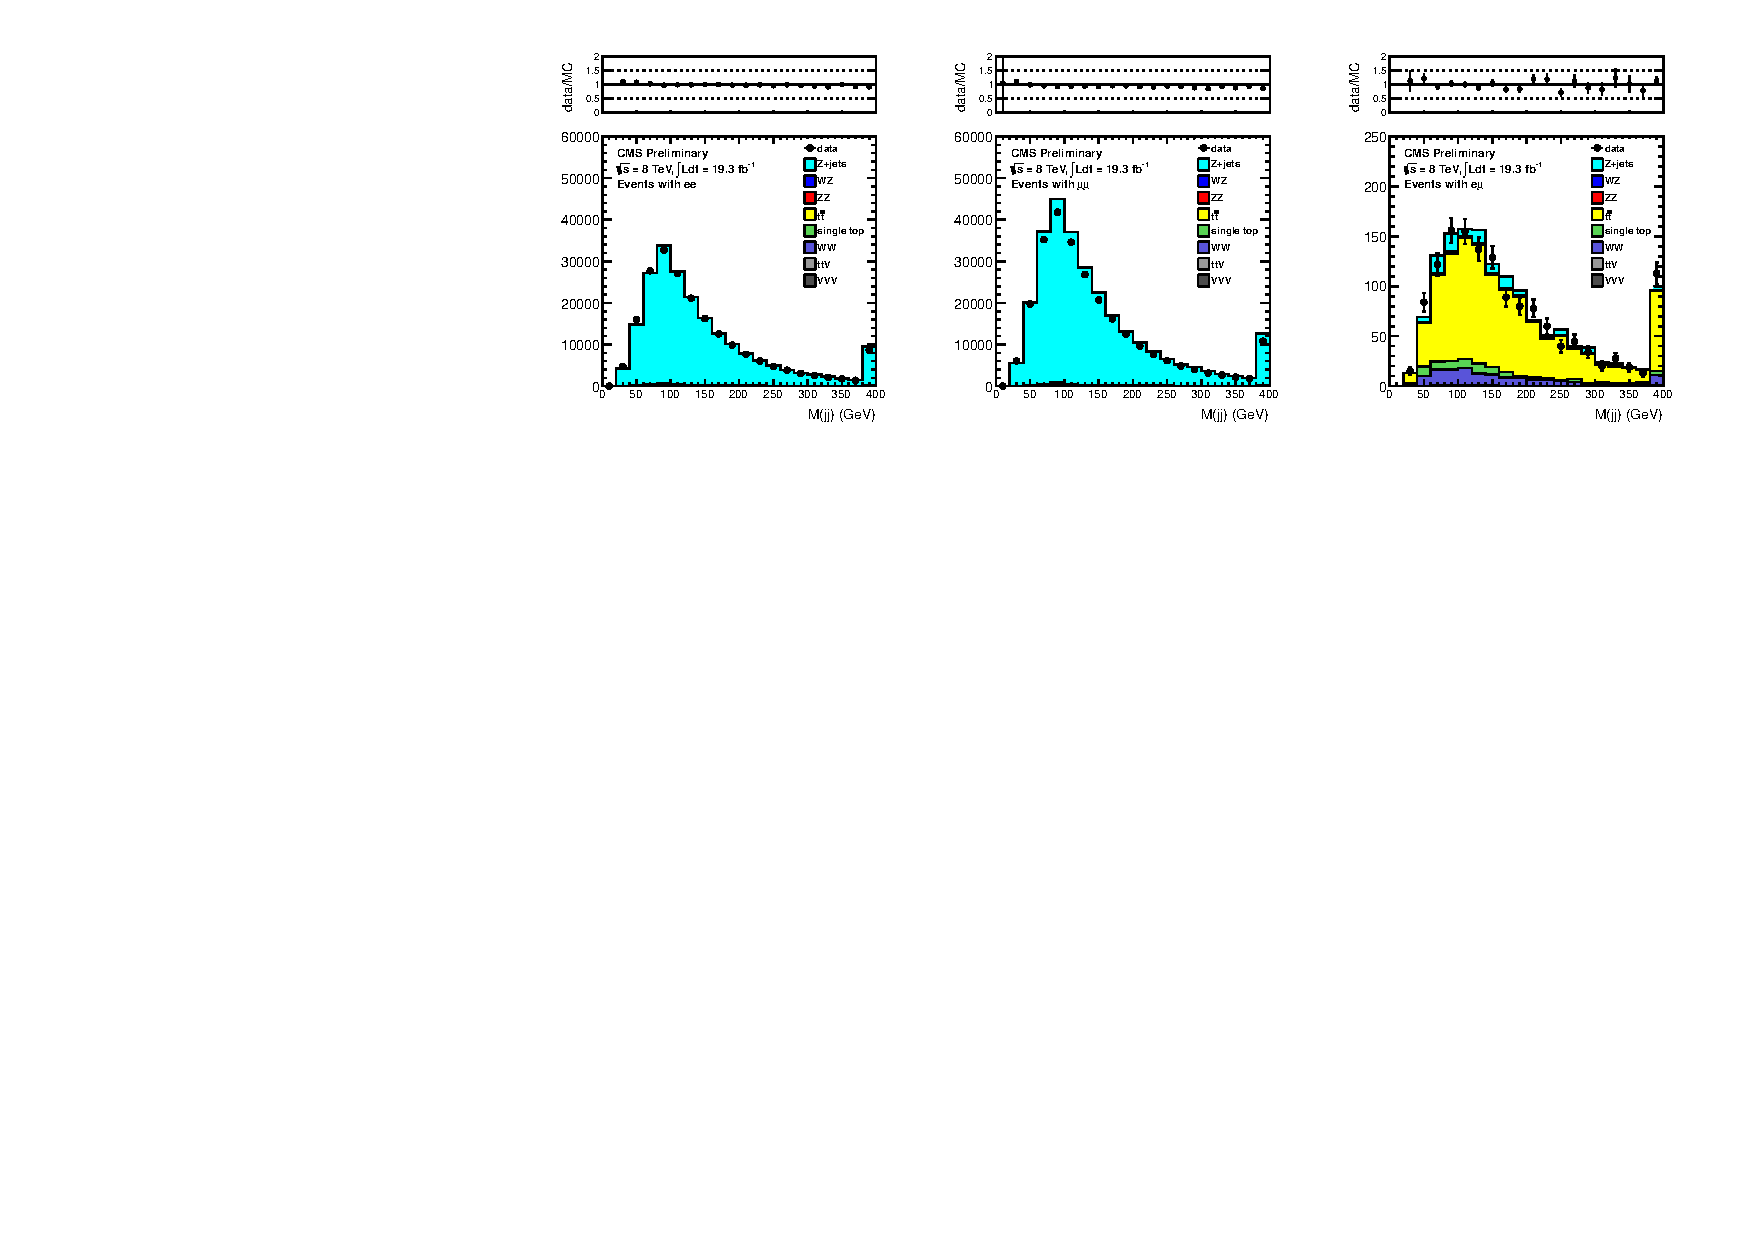
\includegraphics[width=1.0\linewidth]{plots/mjj_targeted_19fb.pdf}
	\caption{
	  \label{fig:mjj}\protect 
Distributions of dijet mass for the targeted preselection in the ee (left), $\mu\mu$ (middle) and e$\mu$ (right) final state.
}                   
  \end{center}
\end{figure}



%Loading babies at       : ../output/V00-02-00
%-------------------------------------
%USING SKIMMED SAMPLES WITH NJETS >= 2
%-------------------------------------

%Using selection         : ((((((((isdata==0 || (run<197556 || run>198913))&&(((leptype==0 && (ee==1 || isdata==0))||(leptype==1 && (mm==1 || isdata==0)))||(leptype==2 && (em==1||me==1||isdata==0))))&&(csc==0 && hbhe==1 && hcallaser==1 && ecaltp==1 && trkfail==1 && eebadsc==1 && hbhenew==1))&&(lep1.pt()>20.0 && lep2.pt()>20.0))&&(dilmass>15.0))&&(njets>=2))&&(nbcsvm==0))&&(nlep==2))&&(dilmass>81 && dilmass<101)
%Using weight            : weight * 19.3 * trgeff * vtxweight
%Plotting var mjj flavor ee
%compareDataMC : apply trigeff 1
%MC yield VVV 12.21
%MC yield ttV 7.75
%MC yield WW 63.50
%MC yield single top 33.64
%MC yield ttbar 435.66
%MC yield ZZ 859.71
%MC yield WZ 1520.22
%SCALING ZJETS BY 111/946
%MC yield zjets 209451.48
%MC total yield 212384.17
%data yield 209905
%Plotting var mjj flavor mm
%compareDataMC : apply trigeff 1
%Warning in <TROOT::Append>: Replacing existing TH1: htemp (Potential memory leak).
%MC yield VVV 15.69
%MC yield ttV 9.57
%MC yield WW 81.36
%MC yield single top 42.28
%MC yield ttbar 539.62
%MC yield ZZ 1113.63
%MC yield WZ 1955.65
%SCALING ZJETS BY 111/946
%MC yield zjets 281080.79
%MC total yield 284838.59
%data yield 266373
%Plotting var mjj flavor em
%compareDataMC : apply trigeff 1
%Warning in <TROOT::Append>: Replacing existing TH1: htemp (Potential memory leak).
%MC yield VVV 2.59
%MC yield ttV 3.22
%MC yield WW 143.37
%MC yield single top 77.11
%MC yield ttbar 1087.65
%MC yield ZZ 1.32
%MC yield WZ 15.18
%SCALING ZJETS BY 111/946
%MC yield zjets 112.51
%MC total yield 1442.95
%data yield 1417

